\chapter{Graph traversal}

This chapter discusses two fundamental
graph algorithms:
depth-first search and breadth-first search.
Both algorithms are given a starting
node in the graph,
and they visit all nodes that can be reached
from the starting node.
The difference in the algorithms is the order
in which they visit the nodes.

\section{Depth-first search}

\index{depth-first search}

\key{Depth-first search} (DFS)
is a straightforward graph traversal technique.
The algorithm begins at a starting node,
and proceeds to all other nodes that are
reachable from the starting node using
the edges in the graph.

Depth-first search always follows a single
path in the graph as long as it finds
new nodes.
After this, it returns to previous
nodes and begins to explore other parts of the graph.
The algorithm keeps track of visited nodes,
so that it processes each node only once.

\subsubsection*{Example}

Let us consider how depth-first search processes
the following graph:
\begin{center}
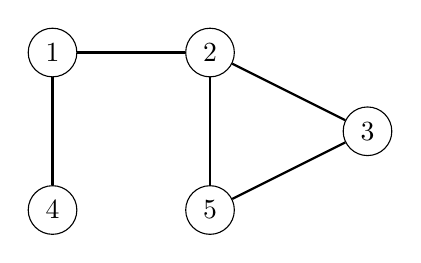
\begin{tikzpicture}
\node[draw, circle] (1) at (1,5) {$1$};
\node[draw, circle] (2) at (3,5) {$2$};
\node[draw, circle] (3) at (5,4) {$3$};
\node[draw, circle] (4) at (1,3) {$4$};
\node[draw, circle] (5) at (3,3) {$5$};

\path[draw,thick,-] (1) -- (2);
\path[draw,thick,-] (2) -- (3);
\path[draw,thick,-] (1) -- (4);
\path[draw,thick,-] (3) -- (5);
\path[draw,thick,-] (2) -- (5);
\end{tikzpicture}
\end{center}
We may begin the search at any node in the graph,
but we will now begin the search at node 1.

The search first proceeds to node 2:
\begin{center}
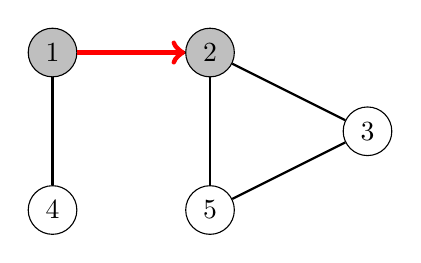
\begin{tikzpicture}
\node[draw, circle,fill=lightgray] (1) at (1,5) {$1$};
\node[draw, circle,fill=lightgray] (2) at (3,5) {$2$};
\node[draw, circle] (3) at (5,4) {$3$};
\node[draw, circle] (4) at (1,3) {$4$};
\node[draw, circle] (5) at (3,3) {$5$};

\path[draw,thick,-] (1) -- (2);
\path[draw,thick,-] (2) -- (3);
\path[draw,thick,-] (1) -- (4);
\path[draw,thick,-] (3) -- (5);
\path[draw,thick,-] (2) -- (5);

\path[draw=red,thick,->,line width=2pt] (1) -- (2);
\end{tikzpicture}
\end{center}
After this, nodes 3 and 5 will be visited:
\begin{center}
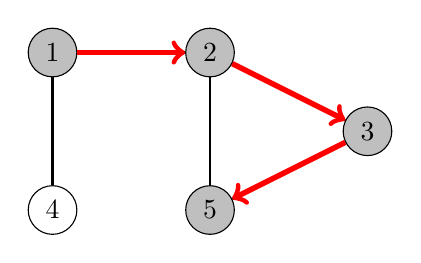
\begin{tikzpicture}
\node[draw, circle,fill=lightgray] (1) at (1,5) {$1$};
\node[draw, circle,fill=lightgray] (2) at (3,5) {$2$};
\node[draw, circle,fill=lightgray] (3) at (5,4) {$3$};
\node[draw, circle] (4) at (1,3) {$4$};
\node[draw, circle,fill=lightgray] (5) at (3,3) {$5$};

\path[draw,thick,-] (1) -- (2);
\path[draw,thick,-] (2) -- (3);
\path[draw,thick,-] (1) -- (4);
\path[draw,thick,-] (3) -- (5);
\path[draw,thick,-] (2) -- (5);

\path[draw=red,thick,->,line width=2pt] (1) -- (2);
\path[draw=red,thick,->,line width=2pt] (2) -- (3);
\path[draw=red,thick,->,line width=2pt] (3) -- (5);
\end{tikzpicture}
\end{center}
The neighbors of node 5 are 2 and 3,
but the search has already visited both of them,
so it is time to return to previous nodes.
Also the neighbors of nodes 3 and 2
have been visited, so we next move
from node 1 to node 4:
\begin{center}
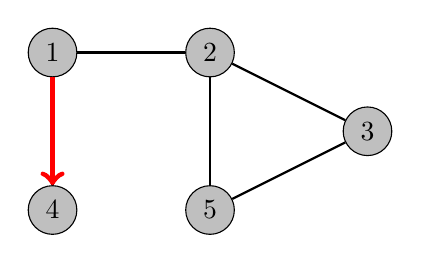
\begin{tikzpicture}
\node[draw, circle,fill=lightgray] (1) at (1,5) {$1$};
\node[draw, circle,fill=lightgray] (2) at (3,5) {$2$};
\node[draw, circle,fill=lightgray] (3) at (5,4) {$3$};
\node[draw, circle,fill=lightgray] (4) at (1,3) {$4$};
\node[draw, circle,fill=lightgray] (5) at (3,3) {$5$};

\path[draw,thick,-] (1) -- (2);
\path[draw,thick,-] (2) -- (3);
\path[draw,thick,-] (1) -- (4);
\path[draw,thick,-] (3) -- (5);
\path[draw,thick,-] (2) -- (5);

\path[draw=red,thick,->,line width=2pt] (1) -- (4);
\end{tikzpicture}
\end{center}
After this, the search terminates because it has visited
all nodes.

The time complexity of depth-first search is $O(n+m)$
where $n$ is the number of nodes and $m$ is the
number of edges,
because the algorithm processes each node and edge once.

\subsubsection*{Implementation}

Depth-first search can be conveniently
implemented using recursion.
The following function \texttt{dfs} begins
a depth-first search at a given node.
The function assumes that the graph is
stored as adjacency lists in an array
\begin{lstlisting}
vector<int> v[N];
\end{lstlisting}
and also maintains an array
\begin{lstlisting}
bool visited[N];
\end{lstlisting}
that keeps track of the visited nodes.
Initially, each array value is \texttt{false},
and when the search arrives at node $s$,
the value of \texttt{visited}[$s$] becomes \texttt{true}.
The function can be implemented as follows:
\begin{lstlisting}
void dfs(int s) {
    if (visited[s]) return;
    visited[s] = true;
    // process node s
    for (auto u: v[s]) {
        dfs(u);
    }
}
\end{lstlisting}

\section{Breadth-first search}

\index{breadth-first search}

\key{Breadth-first search} (BFS) visits the nodes
in increasing order of their distance
from the starting node.
Thus, we can calculate the distance
from the starting node to all other
nodes using breadth-first search.
However, breadth-first search is more difficult
to implement than depth-first search.

Breadth-first search goes through the nodes
one level after another.
First the search explores the nodes whose
distance from the starting node is 1,
then the nodes whose distance is 2, and so on.
This process continues until all nodes
have been visited.

\subsubsection*{Example}

Let us consider how the algorithm processes
the following graph:

\begin{center}
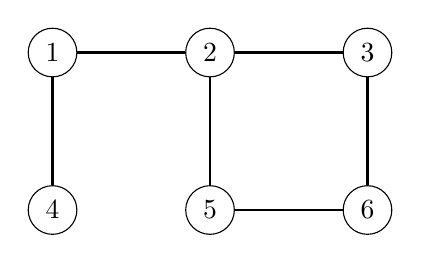
\begin{tikzpicture}
\node[draw, circle] (1) at (1,5) {$1$};
\node[draw, circle] (2) at (3,5) {$2$};
\node[draw, circle] (3) at (5,5) {$3$};
\node[draw, circle] (4) at (1,3) {$4$};
\node[draw, circle] (5) at (3,3) {$5$};
\node[draw, circle] (6) at (5,3) {$6$};


\path[draw,thick,-] (1) -- (2);
\path[draw,thick,-] (2) -- (3);
\path[draw,thick,-] (1) -- (4);
\path[draw,thick,-] (3) -- (6);
\path[draw,thick,-] (2) -- (5);
\path[draw,thick,-] (5) -- (6);
\end{tikzpicture}
\end{center}
Suppose again that the search begins at node 1.
First, we process all nodes that can be reached
from node 1 using a single edge:
\begin{center}
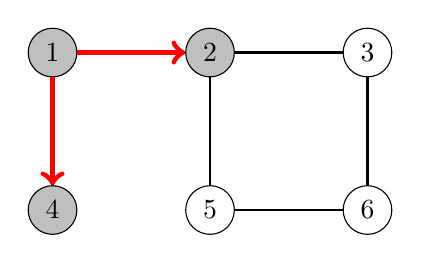
\begin{tikzpicture}
\node[draw, circle,fill=lightgray] (1) at (1,5) {$1$};
\node[draw, circle,fill=lightgray] (2) at (3,5) {$2$};
\node[draw, circle] (3) at (5,5) {$3$};
\node[draw, circle,fill=lightgray] (4) at (1,3) {$4$};
\node[draw, circle] (5) at (3,3) {$5$};
\node[draw, circle] (6) at (5,3) {$6$};

\path[draw,thick,-] (1) -- (2);
\path[draw,thick,-] (2) -- (3);
\path[draw,thick,-] (1) -- (4);
\path[draw,thick,-] (3) -- (6);
\path[draw,thick,-] (2) -- (5);
\path[draw,thick,-] (5) -- (6);

\path[draw,thick,-] (1) -- (2);
\path[draw,thick,-] (2) -- (3);
\path[draw,thick,-] (1) -- (4);
\path[draw,thick,-] (2) -- (5);

\path[draw=red,thick,->,line width=2pt] (1) -- (2);
\path[draw=red,thick,->,line width=2pt] (1) -- (4);
\end{tikzpicture}
\end{center}
After this, we proceed to nodes 3 and 5:
\begin{center}
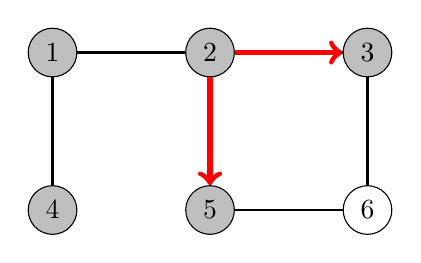
\begin{tikzpicture}
\node[draw, circle,fill=lightgray] (1) at (1,5) {$1$};
\node[draw, circle,fill=lightgray] (2) at (3,5) {$2$};
\node[draw, circle,fill=lightgray] (3) at (5,5) {$3$};
\node[draw, circle,fill=lightgray] (4) at (1,3) {$4$};
\node[draw, circle,fill=lightgray] (5) at (3,3) {$5$};
\node[draw, circle] (6) at (5,3) {$6$};

\path[draw,thick,-] (1) -- (2);
\path[draw,thick,-] (2) -- (3);
\path[draw,thick,-] (1) -- (4);
\path[draw,thick,-] (3) -- (6);
\path[draw,thick,-] (2) -- (5);
\path[draw,thick,-] (5) -- (6);

\path[draw,thick,-] (1) -- (2);
\path[draw,thick,-] (2) -- (3);
\path[draw,thick,-] (1) -- (4);
\path[draw,thick,-] (2) -- (5);

\path[draw=red,thick,->,line width=2pt] (2) -- (3);
\path[draw=red,thick,->,line width=2pt] (2) -- (5);
\end{tikzpicture}
\end{center}
Finally, we visit node 6:
\begin{center}
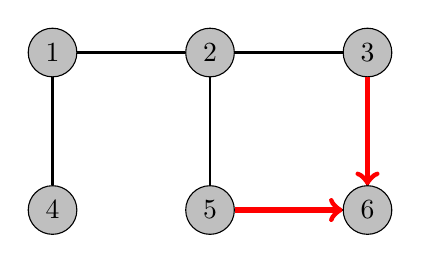
\begin{tikzpicture}
\node[draw, circle,fill=lightgray] (1) at (1,5) {$1$};
\node[draw, circle,fill=lightgray] (2) at (3,5) {$2$};
\node[draw, circle,fill=lightgray] (3) at (5,5) {$3$};
\node[draw, circle,fill=lightgray] (4) at (1,3) {$4$};
\node[draw, circle,fill=lightgray] (5) at (3,3) {$5$};
\node[draw, circle,fill=lightgray] (6) at (5,3) {$6$};

\path[draw,thick,-] (1) -- (2);
\path[draw,thick,-] (2) -- (3);
\path[draw,thick,-] (1) -- (4);
\path[draw,thick,-] (3) -- (6);
\path[draw,thick,-] (2) -- (5);
\path[draw,thick,-] (5) -- (6);

\path[draw,thick,-] (1) -- (2);
\path[draw,thick,-] (2) -- (3);
\path[draw,thick,-] (1) -- (4);
\path[draw,thick,-] (2) -- (5);

\path[draw=red,thick,->,line width=2pt] (3) -- (6);
\path[draw=red,thick,->,line width=2pt] (5) -- (6);
\end{tikzpicture}
\end{center}
Now we have calculated the distances
from the starting node to all nodes in the graph.
The distances are as follows:

\begin{tabular}{ll}
\\
node & distance \\
\hline
1 & 0 \\
2 & 1 \\
3 & 2 \\
4 & 1 \\
5 & 2 \\
6 & 3 \\
\\
\end{tabular}

Like in depth-first search,
the time complexity of breadth-first search
is $O(n+m)$ where $n$ is the number of nodes
and $m$ is the number of edges.

\subsubsection*{Implementation}

Breadth-first search is more difficult
to implement than depth-first search,
because the algorithm visits nodes
in different parts of the graph.
A typical implementation is based on
a queue that contains nodes.
At each step, the next node in the queue
will be processed.

The following code assumes that the graph is stored
as adjacency lists and maintains the following
data structures:
\begin{lstlisting}
queue<int> q;
bool visited[N];
int distance[N];
\end{lstlisting}

The queue \texttt{q}
contains the nodes in increasing order
of their distance.
New nodes are always added to the end
of the queue, and the node at the beginning
of the queue is the next node to be processed.
The array \texttt{visited} indicates
which nodes the search has already visited,
and the array \texttt{distance} will contain the
distances to all nodes in the graph.

The search can be implemented as follows,
starting at node $x$:
\begin{lstlisting}
visited[x] = true;
distance[x] = 0;
q.push(x);
while (!q.empty()) {
    int s = q.front(); q.pop();
    // process node s
    for (auto u : v[s]) {
        if (visited[u]) continue;
        visited[u] = true;
        distance[u] = distance[s]+1;
        q.push(u);
    }
}
\end{lstlisting}

\section{Applications}

Using the graph traversal algorithms,
we can check many properties of the graph.
Usually, either depth-first search or
bredth-first search can be used,
but in practice, depth-first search
is a better choice, because it is
easier to implement.
In the following applications we will
assume that the graph is undirected.

\subsubsection{Connectivity check}

\index{connected graph}

A graph is connected if there is a path
between any two nodes in the graph.
Thus, we can check if a graph is connected
by choosing an arbitrary node and
finding out if we can reach all other nodes.

For example, in the graph
\begin{center}
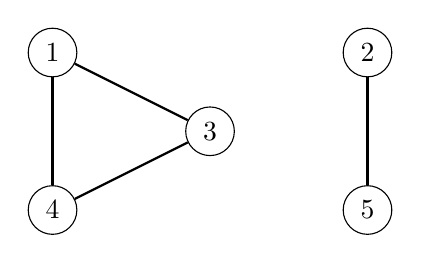
\begin{tikzpicture}
\node[draw, circle] (2) at (7,5) {$2$};
\node[draw, circle] (1) at (3,5) {$1$};
\node[draw, circle] (3) at (5,4) {$3$};
\node[draw, circle] (5) at (7,3) {$5$};
\node[draw, circle] (4) at (3,3) {$4$};

\path[draw,thick,-] (1) -- (3);
\path[draw,thick,-] (1) -- (4);
\path[draw,thick,-] (3) -- (4);
\path[draw,thick,-] (2) -- (5);
\end{tikzpicture}
\end{center}
a depth-first search from node $1$ visits
the following nodes:
\begin{center}
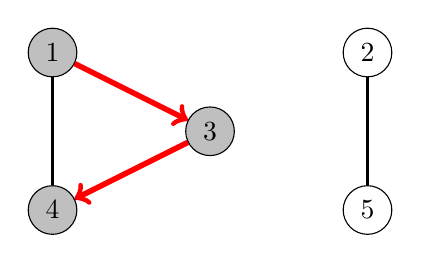
\begin{tikzpicture}
\node[draw, circle] (2) at (7,5) {$2$};
\node[draw, circle,fill=lightgray] (1) at (3,5) {$1$};
\node[draw, circle,fill=lightgray] (3) at (5,4) {$3$};
\node[draw, circle] (5) at (7,3) {$5$};
\node[draw, circle,fill=lightgray] (4) at (3,3) {$4$};

\path[draw,thick,-] (1) -- (3);
\path[draw,thick,-] (1) -- (4);
\path[draw,thick,-] (3) -- (4);
\path[draw,thick,-] (2) -- (5);

\path[draw=red,thick,->,line width=2pt] (1) -- (3);
\path[draw=red,thick,->,line width=2pt] (3) -- (4);

\end{tikzpicture}
\end{center}

Since the search did not visit all the nodes,
we can conclude that the graph is not connected.
In a similar way, we can also find all connected components
of a graph by iterating through the nodes and always
starting a new depth-first search if the current node
does not belong to any component yet.

\subsubsection{Finding cycles}

\index{cycle}

A graph contains a cycle if during a graph traversal,
we find a node whose neighbor (other than the
previous node in the current path) has already been
visited.
For example, the graph
\begin{center}
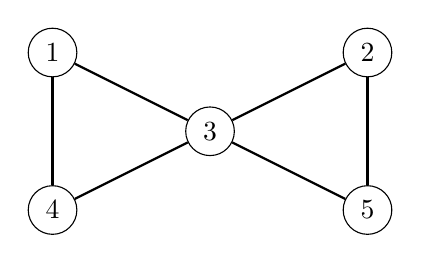
\begin{tikzpicture}
\node[draw, circle] (2) at (7,5) {$2$};
\node[draw, circle] (1) at (3,5) {$1$};
\node[draw, circle] (3) at (5,4) {$3$};
\node[draw, circle] (5) at (7,3) {$5$};
\node[draw, circle] (4) at (3,3) {$4$};

\path[draw,thick,-] (1) -- (3);
\path[draw,thick,-] (1) -- (4);
\path[draw,thick,-] (3) -- (4);
\path[draw,thick,-] (2) -- (5);
\path[draw,thick,-] (2) -- (3);
\path[draw,thick,-] (3) -- (5);
\end{tikzpicture}
\end{center}
contains two cycles and we can find one
of them as follows:
\begin{center}
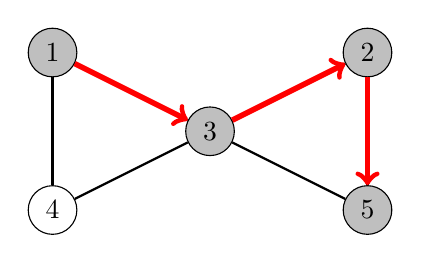
\begin{tikzpicture}
\node[draw, circle,fill=lightgray] (2) at (7,5) {$2$};
\node[draw, circle,fill=lightgray] (1) at (3,5) {$1$};
\node[draw, circle,fill=lightgray] (3) at (5,4) {$3$};
\node[draw, circle,fill=lightgray] (5) at (7,3) {$5$};
\node[draw, circle] (4) at (3,3) {$4$};

\path[draw,thick,-] (1) -- (3);
\path[draw,thick,-] (1) -- (4);
\path[draw,thick,-] (3) -- (4);
\path[draw,thick,-] (2) -- (5);
\path[draw,thick,-] (2) -- (3);
\path[draw,thick,-] (3) -- (5);

\path[draw=red,thick,->,line width=2pt] (1) -- (3);
\path[draw=red,thick,->,line width=2pt] (3) -- (2);
\path[draw=red,thick,->,line width=2pt] (2) -- (5);

\end{tikzpicture}
\end{center}
When we move from
node 2 to node 5 it turns out
that the neighbor 3 has already been visited.
Thus, the graph contains a cycle that goes through node 3,
for example, $3 \rightarrow 2 \rightarrow 5 \rightarrow 3$.

Another way to find out whether a graph contains a cycle
is to simply calculate the number of nodes and edges
in every component.
If a component contains $c$ nodes and no cycle,
it must contain exactly $c-1$ edges
(so it has to be a tree).
If there are $c$ or more edges, the component
surely contains a cycle.

\subsubsection{Bipartiteness check}

\index{bipartite graph}

A graph is bipartite if its nodes can be colored
using two colors so that there are no adjacent
nodes with the same color.
It is surprisingly easy to check if a graph
is bipartite using graph traversal algorithms.

The idea is to color the starting node blue,
all its neighbors red, all their neighbors blue, and so on.
If at some point of the search we notice that
two adjacent nodes have the same color,
this means that the graph is not bipartite.
Otherwise the graph is bipartite and one coloring
has been found.

For example, the graph
\begin{center}
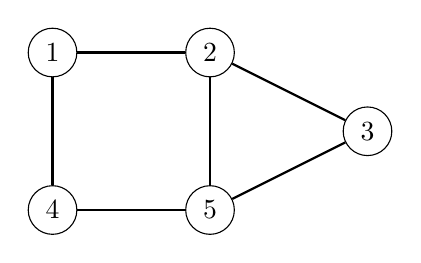
\begin{tikzpicture}
\node[draw, circle] (2) at (5,5) {$2$};
\node[draw, circle] (1) at (3,5) {$1$};
\node[draw, circle] (3) at (7,4) {$3$};
\node[draw, circle] (5) at (5,3) {$5$};
\node[draw, circle] (4) at (3,3) {$4$};

\path[draw,thick,-] (1) -- (2);
\path[draw,thick,-] (2) -- (5);
\path[draw,thick,-] (5) -- (4);
\path[draw,thick,-] (4) -- (1);
\path[draw,thick,-] (2) -- (3);
\path[draw,thick,-] (5) -- (3);
\end{tikzpicture}
\end{center}
is not bipartite, because a search from node 1
proceeds as follows:
\begin{center}
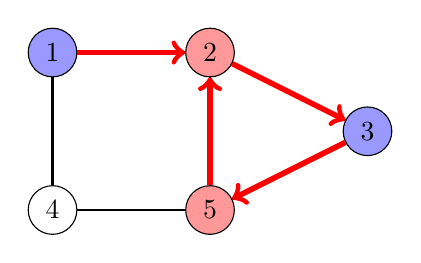
\begin{tikzpicture}
\node[draw, circle,fill=red!40] (2) at (5,5) {$2$};
\node[draw, circle,fill=blue!40] (1) at (3,5) {$1$};
\node[draw, circle,fill=blue!40] (3) at (7,4) {$3$};
\node[draw, circle,fill=red!40] (5) at (5,3) {$5$};
\node[draw, circle] (4) at (3,3) {$4$};

\path[draw,thick,-] (1) -- (2);
\path[draw,thick,-] (2) -- (5);
\path[draw,thick,-] (5) -- (4);
\path[draw,thick,-] (4) -- (1);
\path[draw,thick,-] (2) -- (3);
\path[draw,thick,-] (5) -- (3);

\path[draw=red,thick,->,line width=2pt] (1) -- (2);
\path[draw=red,thick,->,line width=2pt] (2) -- (3);
\path[draw=red,thick,->,line width=2pt] (3) -- (5);
\path[draw=red,thick,->,line width=2pt] (5) -- (2);
\end{tikzpicture}
\end{center}
We notice that the color or both nodes 2 and 5
is red, while they are adjacent nodes in the graph.
Thus, the graph is not bipartite.

This algorithm always works, because when there
are only two colors available,
the color of the starting node in a component
determines the colors of all other nodes in the component.
It does not make any difference whether the
starting node is red or blue.

Note that in the general case,
it is difficult to find out if the nodes
in a graph can be colored using $k$ colors
so that no adjacent nodes have the same color.
Even when $k=3$, no efficient algorithm is known
but the problem is NP-hard.
